\documentclass[../main.tex]{subfiles}
\graphicspath{
    {"../img/"}
    {"img/"}
}

\begin{document}
    Chcemy wygenerować wzór na zamianę zmiennych.
    Dawno dawno temu mogliśmy zrobić tak:
    \[
    \int_2^4 2xe^{x^2}dx =  \mid x^2 = t, 2xdx = dt  \mid=  \int_4^{16}e^{t}dt
    .\]
    Czyli w ogólności
    \[
        \int_{\varphi(a)}^{\varphi(b)}f(x)dx = \int_a^b f(\varphi(t))\varphi'(t)dt
    .\]
    Jak weźmiemy całkę
    \[
        \int f(x,y) dxdy = \int dx \int f(x,y)dy = \mid r=\sqrt{x^2+y^2} , \varphi = arctg(\frac{y}{x})   \mid =  \int dr \int d  \varphi f(r,\varphi) ??
    .\]
    \begin{figure}[h]
        \centering
        \includegraphics[width=0.8\textwidth]{fig_45}
        \caption{zmieniamy zmienne pojedynczo a nie jednocześnie $(x,y)\to (x,\varphi)\to (r,\varphi)$}
    \end{figure}
    \begin{align*}
    &\int dx \int dy f(x,y) = \Vert y = x \tg \varphi, dy = \frac{x}{\cos^2 \varphi}d \varphi \Vert = \int dx \int \frac{x}{\cos^2 \varphi} \varphi f(x,y(x,\varphi))= \\
    &=\Vert x=r \cos \varphi, dx =dr \cos \varphi \Vert = \int d \varphi \int \frac{dr \cos\varphi r \cos \varphi}{\cos^2 \varphi} f(x(r,\varphi), y(x(r,\varphi))) =\\
    &= \int d \varphi \int dr f(r,\varphi) r \text{, czyli } "??" = r
    .\end{align*}
    To teraz w drugą stronę. ($y\to r$), ( $x\to \varphi$ )
    \begin{align*}
        &\int \int f(x,y) dxdy = \Vert y = \sqrt{r^2 - x^2} , dy = \frac{2r dr}{2 \sqrt{r^2-x^2} } \Vert = \\
        &= \int dx \int \frac{r dr}{\sqrt{r^2 - x^2} } f(x,y(x,r)) = \Vert x=r \cos \varphi, dx = -r \sin\varphi d\varphi \Vert = \\
        &=-\int dr \int \frac{r \sin\varphi d \varphi r}{\sqrt{r^2 - x^2} } f(x(r,\varphi),y(x(r,\varphi),r)) = \\
        &= -\int dr r^2 \int d\varphi \frac{\sin\varphi f(r,\varphi)}{\sqrt{r^2 - r^2 \cos^2 \varphi} } = -\int dr \int d\varphi f(r,\varphi) r
    .\end{align*}
    Dostaliśmy prawie to co trzeba ($r$ ). Tylko wpadł jakiś dziwny minus. Podobno minus zniknie gdy doprowadzimy do porządku granice zmiennej $\varphi$, bo $x = r \cos \varphi$ a $\cos$ jest malejący w tym przedziale. (tablica dalej nie działa - minęły 3 miesiące - z marsa by już doszła więc wysyłają pewnie z Saturna - MK$\texttrademark$)

    Niech $\psi \begin{bmatrix} r\\\varphi \end{bmatrix} \to \begin{bmatrix} r \cos \varphi\\ r \sin \varphi \end{bmatrix}  $.
    \begin{align*}
        &\psi' = \begin{bmatrix} \cos \varphi &- r \sin \varphi\\ \sin \varphi & r \cos \varphi \end{bmatrix}\\
        &\Vert \psi' \Vert = r\cos^2 \varphi - (-r\sin^2 \varphi) = r
    .\end{align*}
    Chcemy pokazać, że jeżeli $\varphi: A\to A$, $A\subset\mathbb{R}^n$, $\varphi$ - klasy $\mathcal{C}^1, \varphi^{-1}$ - klasy $\mathcal{C}^1$, to możemy przedstawić $\varphi$ jako złożenie dwóch transformacji, z których pierwsza nie zmienia $n-1$ zmiennych a druga nie zmienia $1$ zmiennej (transformacje pierwotne/prymitywne albo inne ubogacające nazwy).
    \begin{proof}
        (coś w rodzaju dowodu)\\
        $\varphi$ możemy przedstawić jako
        \[
            \varphi \begin{bmatrix} t_1\\ \vdots \\ t_n \end{bmatrix} \to \begin{bmatrix} \varphi_1(t_1,\ldots,t_n)\\ \vdots \\ \varphi_n(t_1,\ldots,t_n) \end{bmatrix} = \begin{bmatrix} x_1 \\ \vdots \\ x_n \end{bmatrix}
        .\]
        \begin{pytanie}
            Czy istnieje odwzorowanie $\Theta^{-1}: A\to A$ takie, że
            \[
                \Theta = \begin{bmatrix} t_1\\ \vdots \\ t_n \end{bmatrix} = \begin{bmatrix} t_1 \\ \vdots \\ t_{j-1} \\ \varphi_j(t_1,\ldots,t_n)\\ t_{j+1} \\ \vdots \\ t_n \end{bmatrix} = \begin{bmatrix} x_1 \\ \vdots \\ x_{j-1} \\ x_j \\ x_{j+1} \\ \vdots \\ x_n \end{bmatrix}
            .\]
            ($t_{i\neq j}$ ) mogą zostać zamiast zamieniać je na $x_i$.
            Dlaczego interesuje nas czy istnieje funkcja odwrotna? Bo jeżeli istnieje, to możemy zapisać
            \[
                \varphi = \varphi \circ \Theta^{-1} \circ \Theta = \left(\varphi \circ \Theta^{-1}\right) \circ \Theta
            .\]
        \end{pytanie}
        Wiemy, że $\varphi$ - klasy $\mathcal{C}^1$ i $\varphi^{-1}$ - klasy $\mathcal{C}^1$ i $\varphi: A\to A$. Mamy twierdzenie o lokalnej odwracalności!\\
        $det \varphi' \neq 0$ , czyli w macierzy $\varphi'$ istnieje prznajmniej $1$ element niezerowy. (w rzeczywistości to zawsze będzie trochę więcej - nieśmiały warunek)

        np. $\frac{\partial \varphi^i}{\partial t^i} \neq 0$. Oznacza to, że odwzorowanie
        \[
            \eta : \begin{bmatrix} t_1 \\ t_2 \\ \vdots \\ t_{i-1} \\t_i \\ t_{i+1} \\ \vdots \\ t_n \end{bmatrix} \to \begin{bmatrix} x_1\\ x_2 \\ \vdots \\ x_{j-1} \\ x_j = \varphi^i (t_1,\ldots,t_n) \\ \vdots \\ x_n \end{bmatrix}
        .\]
        Wtedy
        \[
            \eta' = \begin{bmatrix} 1&&&&\\ &1&&& \\ \ldots&\ldots& \frac{\partial \varphi^i}{\partial x^i} &\ldots&\ldots \\ &&&1& \\ &&&&1\end{bmatrix}
        .\]
        i $\det \eta' \neq 0$, więc istnieje $\eta^{-1}$. \\
        Czyli $\varphi = \varphi \circ \eta \circ \eta^{-1} = (\varphi \circ \eta ) \circ \eta^{-1} \quad\Box$
    \end{proof}

    \begin{equation}
        \int_{-1}^{1}dx\int_{-\sqrt{1-x^2} }^{\sqrt{1-x^2} }dy f(x,y) = \int_0^1 r dr \int_0^{2\pi} d\varphi f(r,\varphi)
    \end{equation}
    \begin{tw}
        (O zamianie zmiennych)\\
        Niech $\Theta, \Omega$ - zbiory otwarte w $\mathbb{R}^n$ i $\xi: \Omega\to \Theta$, $f: \Theta\to \mathbb{R}$, $f$ - ograniczona i całkowalna. $\xi$ - klasy $\mathcal{C}^1$ na $\Omega$, $\xi^{-1}$ klasy $\mathcal{C}^{1}$ na $\Theta$. Wtedy
        \begin{equation}
            \int_{\Theta} f(x) dx =  \int_{\Omega} f(\xi(t)) | \det \xi'(t) | dt.
        \end{equation}
        $x=(x^1,\ldots,x^n)\in \Theta, t=(t^1,\ldots,t^n)\in \Omega$
    \end{tw}
    \begin{figure}[h]
        \centering
        \includegraphics[width=0.8\textwidth]{fig_46}
        \caption{$\Omega\to\Theta - f - \mathbb{R}$}
    \end{figure}
    \begin{proof}
        (przez indukcję względem wymiaru przestrzeni)\\
        \begin{itemize}
            \item dla $n=1$ - zrobione w I semetrze.
            \item zakładamy, że prawdziwy jest napis
                \[
                    \int_{A'\subset\mathbb{R}^{n-1}} f(x)dx = \int_{\Omega' \subset\mathbb{R}^{n-1}} f(\xi(t)) | det(\xi'(t)) |, (\xi: \mathbb{R}^{n-1}\to \mathbb{R}^{n-1})
                .\]
        \end{itemize}
        Chcem pokazać, że prawdziwy jest napis
        \[
            \int_{A\subset\mathbb{R}} f(x) dx = \int_{\Omega \subset \mathbb{R}^n} f(\xi(t)) | det(\xi'(t)) |
        .\]
        Uwaga: wartośc bezwzględna oznacza, że musimy uważać przy rozstawianiu granic:\\
        $\left( \int_a^b f \right) $ oznacza, że zakładamy, że $a\le b$. Dowód przeprowadzamy dla $\xi: \Theta\subset\mathbb{R}^n\to \Omega\subset\mathbb{R}^n$ takiego, że $\xi$ nie zamienia jednej zmiennej.
        \begin{obserwacja}
            Niech $K = \left\{ (x,y), x^2+y^2 \le 1 \right\} $, niech $K_a = \left\{ (x,a), x^2+a^2 \le 1 \right\}.$\\
            Wówczas $K = \bigcup_{a\in[-1,1]}K_a$, zatem $\int_K f = \int_{-1}^1 da \int _{K_a} f$

        \end{obserwacja}
    Ostatnio skończyliśmy na kroku $n-1\to n$ i wiemy, że dla $n-1$ wymiarów możemy napisać
    \[
        \int_{A\in \mathbb{R}^{n-1}}f(x)dx = \int_{B\in \mathbb{R}^{n-1}}f(\xi(t)) |\det \xi'|dt
        .\]
    \begin{figure}[h]
        \centering
        \includegraphics[width=0.3\textwidth]{fig_48}
        \caption{Kółko $K$ składamy z kresek $K_a$ i mamy $\int_K f = \int da \int_{K_a} f$}
        \label{fig:fig_48}
    \end{figure}

    \[
        \int_{\Theta} f dx = \int_{\Omega}f(\xi(t))|\det \xi'|dt
    .\]
    Mając zbiór $\Theta$, zdefiniujmy zbiór $\Theta_a$, który jest zbiorem takich $x\in\Theta$, że na miejsca $x_i$ wstawimy wielkość $a$.
    \[
        \Theta_a = \left\{ x\in \mathbb{Q}, x = \left( x^1,x^2,\ldots,x^{i-1},a,x^{i+1},\ldots,x^n \right)  \right\}
    .\]
    \[
        K = \left\{ (x,y), x^2+y^2 = 1 \right\}
    .\]
    \[
        K_a = \left\{ (x,y)\in K, (x,y) = (x,a) \right\}, \left\{ (x,a), x^2+a^2 = 1 \right\}
    .\]
    Oznacza to, że
    \[
        \int_\Theta f dx = \int da \int_{\Theta_a}f(x^1,x^2,\ldots,x^{i-1},a,x^{i+1},\ldots,x^n) dx^1 dx^2 \ldots dx^{i-1} dx^{i+1}\ldots dx^n
    .\]
    Rozważmy $\xi: \Theta \to \Omega$ taką, że
    \[
        \begin{bmatrix} t_1\\ \vdots \\ t_n \end{bmatrix} \to \begin{bmatrix} \xi_1(t_1,\ldots,t_n)\\ \xi_2(t_1,\ldots,t_n) \\ \vdots \\ \xi_{i-1} \\ t_1 \\ \xi_{i+1} \\ \vdots \\ \xi_n(t_1,\ldots,t_n)
    \end{bmatrix} \begin{bmatrix} x^1\\x^1\\ \vdots \\ x^i \\ \vdots \\ x^n \end{bmatrix}
    .\]
    Czyli $\xi$ nie zmienia jednej współrzędnej np.
    $\begin{bmatrix}
        x\\y
    \end{bmatrix}
    \to
    \begin{bmatrix}
        r\\x
    \end{bmatrix}$.\\
    Możemy więc zapisać transformację $\xi_a: \Theta_a\to\Omega_a$

     \[
         \begin{bmatrix} t_1\\ \vdots\\ t_{i-1}\\ t_{i+1} \\ \vdots \\ t_n \end{bmatrix} \to \begin{bmatrix} \xi_1(t_1,\ldots,t_n) \\ \xi_2(t_1,\ldots,t_n) \\ \vdots \\ \xi_{i-1}(\ldots) \\ \xi_{i+1}(\ldots) \\ \vdots \\ \xi_n(t_1,\ldots,t_n)\end{bmatrix}
    .\]
    Wówczas na mocy założenia indukcyjnego wiemy, że
    \begin{align*}
        &\int_{\Theta_a}f(x^1,\ldots,x^{i-1},a,x^{i+1},\ldots,x^n) dx^1 \ldots dx^{i-1} dx^{i+1} \ldots dx^n = \\
        &\int_{\Omega_a} f(t_1,t_2,\ldots,t_{i-1},a,t_{i+1},\ldots,t_n) |\det \xi'_a | dt^1 dt_2 \ldots dt^{i-1} dt^{i+1} \ldots dt^n
    .\end{align*}
    Wówczas
    \begin{align*}
        &\int_{\Theta}f(x^1,\ldots,x^n)dx^n = \int_a da \int_{\Omega_a}f(t_1,\ldots,t_{i-1},a,t_{i+1},\ldots,t_n) |\det \xi'_a| \cdot (\pm 1) dt^1 \ldots dt^{i-1} dt^{i+1} \ldots dt^n\\
        &= \begin{bmatrix} a=t_i \end{bmatrix} =\\
        &= \int_{\Omega} f(t^1,t^2,\ldots,t^n)|\det \xi' | dt^1 \ldots dt^n
.\end{align*}

\[
    \xi' = \begin{bmatrix} \frac{\partial \xi_1}{\partial t_1} & \frac{\partial \xi_2}{\partial t_2} & \ldots && \frac{\partial \xi_n}{\partial t_n}\\ 0 & \ldots & 1 & \ldots & 0 \\ \frac{\partial \xi_n}{\partial t_1} & \ldots &&& \frac{\partial \xi_n}{\partial t_n}  \end{bmatrix}
.\]

    \end{proof}
    \begin{figure}[h]
        \centering
        \includegraphics[width=0.8\textwidth]{fig_47}
    \end{figure}

    \begin{przyklad}
        Policzmy całkę $I = \int_0^{\infty}e^{-x^2}dx$. Nie umiemy. Ale skoro nie umiemy policzyć $I$, to tym bardziej $I^2?$
        \[
            I^2 = \int_0^{\infty}e^{-x^2}dx \int_0^{\infty}e^{-y^2}dy = \int_{\Box} e^{-(x^2+y^2)}
        .\]
        Zamieńmy sobie zmienne: $x = r\cos \varphi,\quad y = r\sin \varphi$. $\psi: \begin{bmatrix} r\\\varphi\end{bmatrix}\to \begin{bmatrix} x\\y \end{bmatrix}  $, $|\psi'| = r$
         Mamy
         \begin{align*}
             &I^2 = \int_0^{\infty}dr \int_0^{\frac{\pi}{2}}d\varphi e^{-r^2}r = \frac{\pi}{2} \lim\limits_{p\to +\infty} \int_0^p dr \cdot e^{-r^2} \cdot r = \frac{\pi}{2} \lim\limits_{p\to\infty} \left[ -\frac{1}{2}e^{-r^2} \right] _0^p\\
             &\frac{\pi}{2}\left[ \lim\limits_{p\to\infty}\left[ -\frac{1}{2}e^{-p^2} \right] - \left[ -\frac{1}{2}e^{(0)^2} \right]  \right] = \frac{\pi}{2} \frac{1}{2} = \frac{\pi}{4}
         \end{align*}
         czyli $I^2 = \frac{\pi}{4} \implies I = \frac{\sqrt{\pi} }{2}$
    \end{przyklad}

\end{document}
